\capitulo{3}{Conceptos teóricos}

El desarrollo del proyecto PrimeBot (Figura 3.1) implica abordar diversos aspectos teóricos con un nivel considerable de complejidad. 
A continuación, se detallan los conceptos teóricos clave que sustentan este proyecto, abordando tanto componentes electrónicos como algoritmos fundamentales.
\begin{figure}[h]
	\centering
	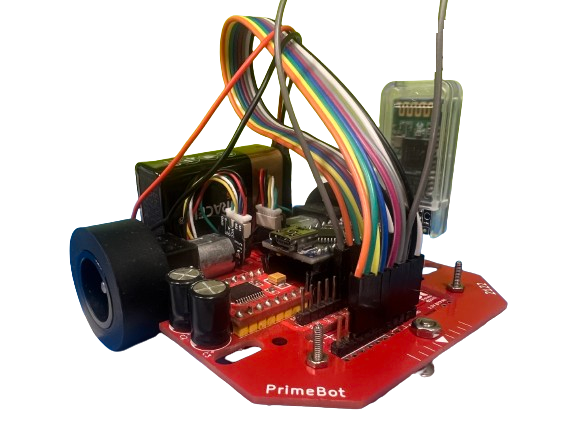
\includegraphics[width=0.5\textwidth]{primebot}
	\caption{PrimeBot}
	\label{fig:3.1}
\end{figure}

PrimeBot se trata de un robot móvil de tracción diferencial ya que dispone de dos ruedas que pueden girar de forma independiente (Figura 3.2).
\begin{figure}[h]
	\centering
	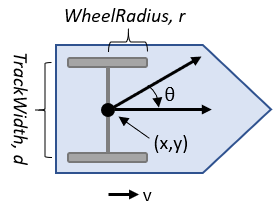
\includegraphics[width=0.25\textwidth]{tracciondiferencial}
	\caption{Modelo de robot de tracción diferencial.}
	\label{fig:3.2}
\end{figure}

\section{Placa de Control}\label{placa-de-control}
PrimeBot está equipado con varios componentes electrónicos esenciales para su funcionamiento y desempeño en las pruebas del ASTI Robotics Challenge. Todo el sistema de PrimeBot está integrado en una Placa de Circuito Impreso (PCB) diseñado específicamente para este proyecto (Figura 3.3) que alberga todos los componentes electrónicos esenciales y facilita su interconexión y gestión.
\begin{figure}[h]
	\centering
	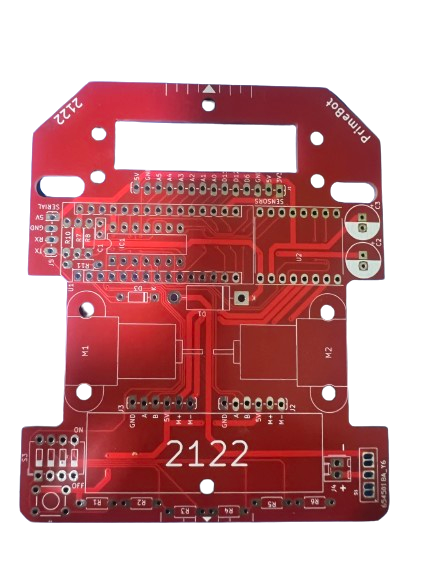
\includegraphics[width=0.20\textwidth]{pcb}
	\caption{PCB}
	\label{fig:3.3}
\end{figure}

\subsection{Arduino Nano Every}\label{arduino-nano}
Arduino Nano Every(Figura 3.4) es un microcontrolador compacto y versátil que actúa como el cerebro de PrimeBot, controlando todos los componentes y ejecutando los programas necesarios para las diferentes pruebas.~\cite{arduinoNanoEvery}
Se ha seleccionado esta placa ya que es el Arduino con el factor de forma más pequeño disponible y tiene un gran número de pines tanto digitales como analógicos para utilizar en todos los sensores que se van a uitilizar en el proyecto.

Además esta placa es una versión mejorada del Arduino Nano convencional, incorporando una mayor cantidad de memoria RAM y memoria Flash que nos permite ejecutar programas más potentes como el que se utiliza en la prueba de la cuadrícula.
\begin{figure}[h]
	\centering
	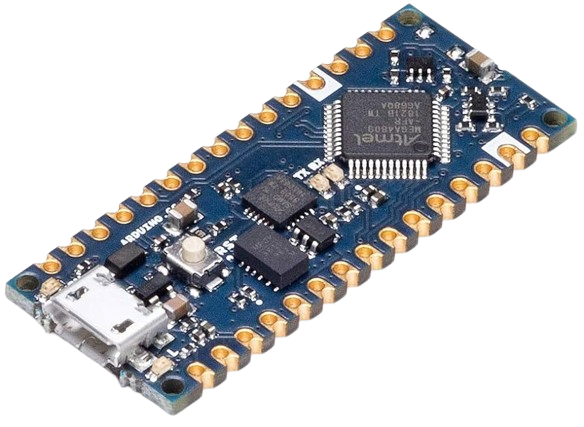
\includegraphics[width=0.25\textwidth]{arduino}
	\caption{Arduino Nano Every}
	\label{fig:3.4}
\end{figure}
\newpage
\subsection{Motores N20}\label{N20}
Motores (Figura 3.5) de corriente continua de alta eficiencia y tamaño compacto, adecuados para aplicaciones que requieren precisión y control.
\begin{figure}[h]
	\centering
	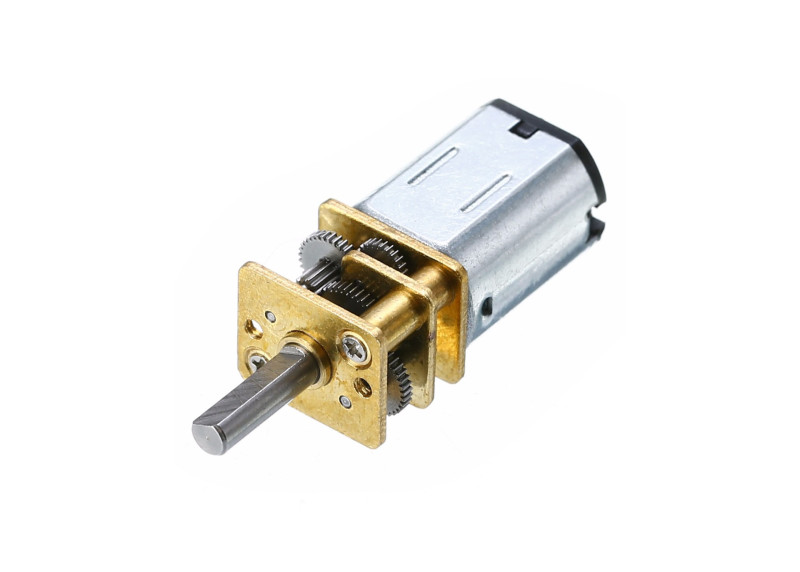
\includegraphics[width=0.25\textwidth]{n20}
	\caption{Motores N20}
	\label{fig:3.5}
\end{figure}


\subsection{Encoders magnéticos}\label{encoders}
Los encoders magnéticos (Figura 3.6) son unos ensores que proporcionan retroalimentación precisa sobre la posición y velocidad de los motores, fundamentales para el control PID.
\begin{figure}[h]
	\centering
	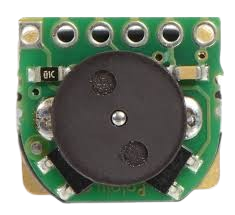
\includegraphics[width=0.2\textwidth]{encoder}
	\caption{Encoders Magnéticos}
	\label{fig:3.6}
\end{figure}

\subsection{Driver de motores TB6612FNG}\label{driver}
Controlador de motores que permite manejar hasta dos motores DC (Figura 3.7), proporcionando una interfaz de control eficiente y protecciones integradas contra sobrecorriente y sobretemperatura.
\begin{figure}[h]
	\centering
	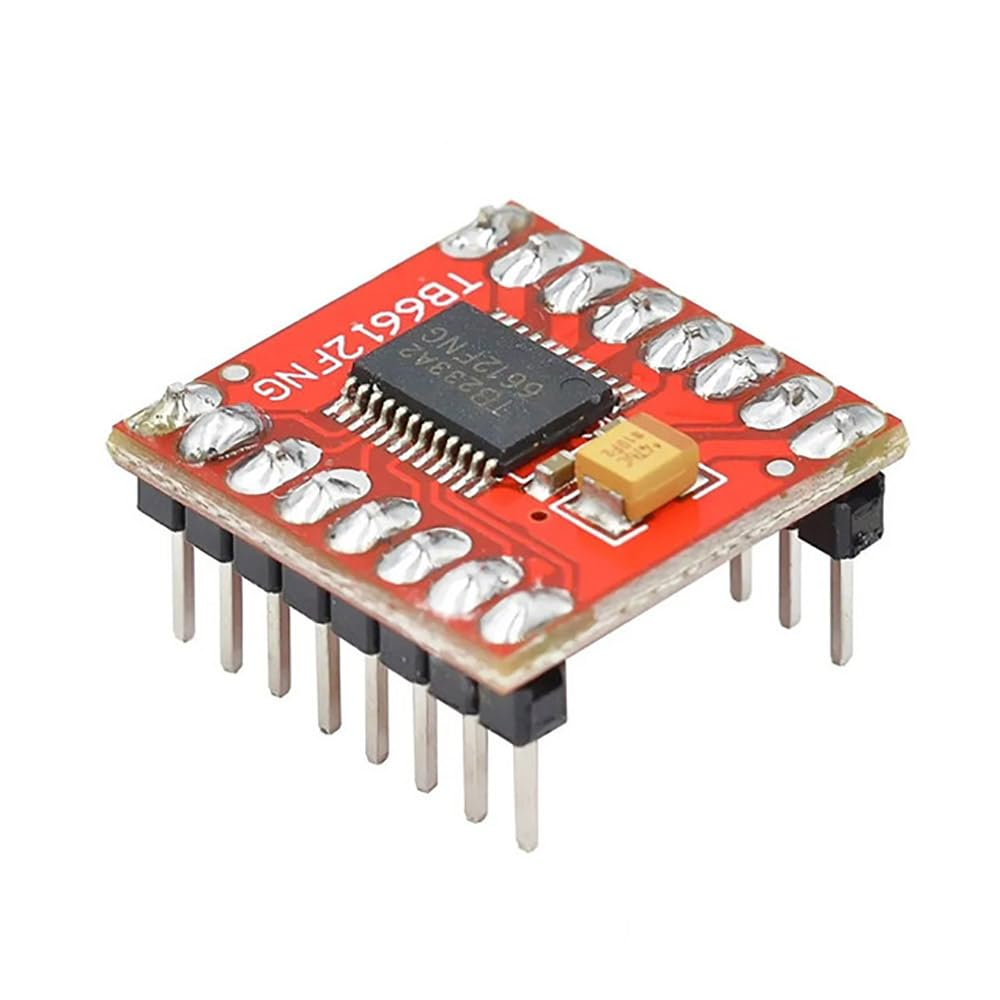
\includegraphics[width=0.2\textwidth]{tb6612fng}
	\caption{Driver de Motores}
	\label{fig:3.7}
\end{figure}

\subsection{Sensores QTR8A}\label{qtr8a}
Sensores de reflectancia utilizados para la detección de líneas en el suelo (Figura 3.8), cruciales para las pruebas de seguimiento de líneas. Estos sensores permiten detectar contrastes entre diferentes superficies, como líneas negras sobre fondos blancos. ~\cite{pololuQTR8A}

\begin{figure}[h]
	\centering
	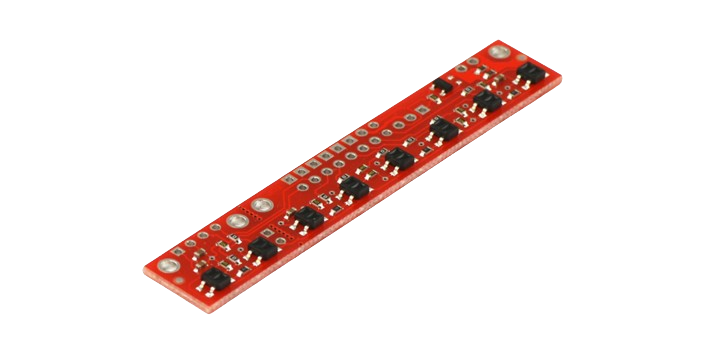
\includegraphics[width=0.5\textwidth]{qtr8a}
	\caption{Sensores de reflectancia QTR-8A}
	\label{fig:3.8}
\end{figure}

\subsection{Pololu OPT3101}\label{opt3101}
Sensores de distancia basados en tiempo de vuelo (ToF) (Figura 3.9) que proporcionan mediciones precisas de distancia, útiles para la navegación y evitación de obstáculos en el entorno del robot. ~\cite{pololuOPT3101}
\begin{figure}[h]
	\centering
	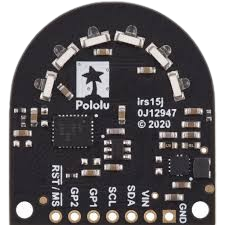
\includegraphics[width=0.5\textwidth]{OPT3101}
	\caption{Sensores de distancia OPT3101}
	\label{fig:3.9}
\end{figure}


\subsection{Selector de posición}\label{selector-de-posicion}
En el PCB de PrimeBot hay un switch mini DIP de 4 posiciones (Figura 3.10) integrado junto a un botón que permite ejecutar el programa correspondiente a la posición seleccionada en el mini DIP.
\begin{figure}[h]
	\centering
	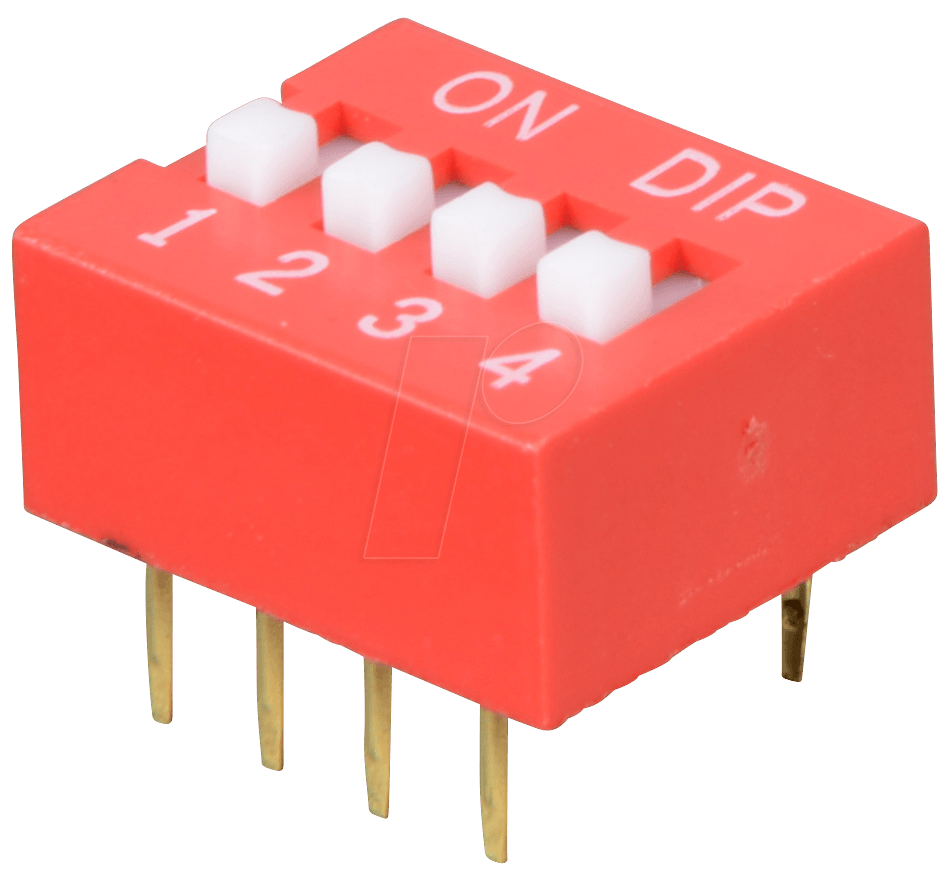
\includegraphics[width=0.25\textwidth]{dip}
	\caption{Switch DIP}
	\label{fig:3.10}
\end{figure}


\subsubsection{Valores del Switch}
El Switch Mini DIP contiene 4 selectores que se pueden mover entre dos posiciones (0 y 1), permitiendo seleccionar desde la posición 0000 hasta la posición 1111, es decir, un total de 15 posiciones diferentes. Esto permite cargar diferentes programas independientes o secciones diferentes de un mismo programa.

El botón situado al lado del Switch proporciona el valor '16' (10000) que el programa 'Main' interpreta como valor de cambio de programa. Esto detiene el programa en ejecución y activa el correspondiente a la nueva posición del switch.

\subsubsection{Uso de Resistencias}
Para que la placa principal de Arduino pueda entender en qué posición está el switch mini DIP, se utilizan una serie de resistencias soldadas en la placa junto a la función de lectura analógica de Arduino. El uso de la lectura analógica de un pin (\emph{AnalogRead()}) dentro de Arduino devuelve un valor de 0 a 1023. Utilizando resistencias de diferentes valores y reflejándolos en el código, Arduino puede interpretar la posición del switch.

El valor de las resistencias es crucial, ya que deben seleccionarse valores bien distanciados para evitar errores en la lectura debido a las tolerancias. Una correcta selección y calibración de estas resistencias asegura una interpretación precisa y fiable de la posición del switch.

En el caso de PrimeBot, para interactuar directamente con el Switch DIP encontramos:
\begin{itemize}
	\item 1 resistencia de 10k ohms
	\item 1 resistencia de 4k7 ohms
	\item 1 resistencia de 2k2 ohms
	\item 1 resistencia de 1k ohms
\end{itemize}

Estos valores están muy distanciados y aproximadamente uno es el doble que el posterior, de esta forma cuando subimos la posición 1 del switch es decir ejecutamos 0001, la resistencia que actúa es la resistencia de 1k ohms y cuando realizamos la lectura correspondiente con \emph{AnalogRead()} obtendremos un valor que será muy diferente al que obtendremos en la posición 0010 que actuará una resistencia de 2k2 ohms y así sucesivamente.
Con el uso de estas resistencias distantes en cuanto a ohms conseguimos realizar lecturas fiables para ejecutar el programa deseado.

\subsection{Integración de Componentes}
El diseño del PCB de PrimeBot está optimizado para integrar todos los componentes necesarios, incluyendo el Arduino Nano, los motores, encoders, sensores y el driver de motores. Esta integración asegura un montaje compacto y ordenado, minimizando las interferencias y facilitando las conexiones.

El PCB también incluye conectores intercambiables para diferentes sensores, lo que permite adaptar fácilmente PrimeBot a las diversas pruebas del ASTI Robotics Challenge. Esta flexibilidad es uno de los puntos fuertes de PrimeBot, permitiendo una rápida configuración y reconfiguración según las necesidades específicas de cada prueba.

\section{Conectividad}\label{conectividad}
PrimeBot incorpora la funcionalidad de conectividad Bluetooth para mejorar la flexibilidad y el control del robot. Esta capacidad permite a los usuarios ajustar los parámetros operativos del robot en tiempo real, sin necesidad de detenerlo ni conectarlo físicamente a un ordenador.

\subsection{Conectividad Bluetooth}
La conectividad Bluetooth en PrimeBot está diseñada para proporcionar instrucciones intuitivas y sencillas para los usuarios. A través de una aplicación compatible o una interfaz serial Bluetooth estándar, los desarrolladores pueden conectarse al robot y modificar configuraciones críticas como las constantes del PID (Proporcional, Integral, Derivativo), la velocidad base y otros parámetros operativos.

\textbf{Uso y Configuración:}
\begin{itemize}
	\item \textbf{Emparejamiento:} Primero, el módulo Bluetooth de PrimeBot debe emparejarse con el dispositivo del usuario (smartphone, tablet, o PC). Este proceso suele implicar buscar dispositivos Bluetooth disponibles, seleccionar PrimeBot y, si es necesario, introducir un código de emparejamiento.
	\item \textbf{Conexión:} Una vez emparejado, se establece una conexión Bluetooth. En este punto, los comandos y datos pueden ser enviados y recibidos.
	\item \textbf{Ajuste de Parámetros:} Mediante comandos simples, el usuario puede ajustar los parámetros operativos. Por ejemplo, enviar 'P+0.1' para aumentar el valor de Kp en 0.1, o 'B+5' para incrementar la velocidad base en 5 unidades.
	\item \textbf{Monitoreo en Tiempo Real:} Los datos del sensor y otros parámetros operativos pueden ser transmitidos de vuelta al dispositivo del usuario, permitiendo el monitoreo en tiempo real y ajustes instantáneos según sea necesario.
\end{itemize}
Esta funcionalidad es especialmente útil durante las competiciones, donde los ajustes rápidos y precisos pueden ser la clave para el éxito. La conectividad Bluetooth facilita también la depuración y el monitoreo del rendimiento del robot, proporcionando una visión inmediata de su estado y comportamiento.


\section{Movimientos y habilidades}\label{movimientos}

\subsection{Algoritmo PID}\label{algoritmo-pid}

Para encontrar un buen equilibrio entre precisión y velocidad el algoritmo utilizado en muchas aplicaciones industriales es el algoritmo PID. ~\cite{ogata2010}

\textbf{El funcionamiento del PID}

El algoritmo PID es un proceso de realimentación en el que un sistema está constantemente recibiendo valores de entrada, en nuestro caso los valores de los sensores.
Con esos valores de entrada el algoritmo PID realiza unos cambios en el sistema que alteran los valores de entrada que va a recibir posteriormente buscando reducir al mínimo el error.

Un algoritmo PID es exitoso cuando se consigue reducir el error al mínimo en todas las lecturas.

Como su nombre indica, el algoritmo PID dispone de tres partes de control principalmente:

\begin{itemize}
	\item \textbf{Parte Proporcional (P):} La parte proporcional es el producto entre la señal del error y la constante proporcional (Kp) proporcionada para que el error se aproxime a cero.
	\item \textbf{Parte Integral (I):} La parte integral tiene como objetivo disminuir el error en estado estacionario y todo lo que no es corregible por la parte proporcional. Se utiliza la constante integral (Ki) como constante a la que multiplicar el error integrado.
	\item \textbf{Parte Derivativa (D):} La parte derivativa tiene en cuenta la tasa de cambio de error proporcionando una acción correctiva basada en la velocidad a la que cambia el error.
\end{itemize}

Además de estas partes, en PrimeBot se incluye también una constante 'Kv' utilizada para optimizar el algoritmo PID en las rectas permitiendo que PrimeBot tenga un mayor rendimiento en zonas donde el error que hay es mínimo aumentando la velocidad.

La fórmula utilizada para el control PID es la siguiente:
\begin{equation*}
	motorSpeedAdjustment = Kp * error + Ki * integral + Kd * derivative
\end{equation*}

\subsection{Seguidor de Líneas}\label{seguidor-lineas}
PrimeBot está diseñado para seguir líneas de manera precisa utilizando el algoritmo PID. 
A continuación, se describen las características, parámetros ajustables y el uso de Bluetooth para el seguidor de líneas.
\subsubsection{Características del Seguidor de Líneas}\label{caracteristicas-seguidor-lineas}

PrimeBot utiliza sensores de reflectancia QTR8A para detectar la línea en el suelo. Estos sensores detectan el contraste entre diferentes superficies, como líneas negras sobre fondos blancos, y envían esta información al microcontrolador. El algoritmo PID procesa estos datos para ajustar la velocidad de los motores y mantener al robot en la trayectoria deseada.

\subsubsection{Parámetros Ajustables por Bluetooth}

Para facilitar el control y ajuste del seguidor de líneas, varios parámetros pueden ser modificados en tiempo real mediante una conexión Bluetooth:
\begin{itemize}
\item \textbf{Constantes PID (Kp, Ki, Kd):} Permiten ajustar la respuesta del algoritmo PID para mejorar el seguimiento de líneas y la estabilidad del robot.
\item \textbf{Constante Kv:} Optimiza el rendimiento en tramos rectos, aumentando la velocidad cuando el error es mínimo.
\item \textbf{Velocidad Base (BaseSpeed):} Ajusta la velocidad base de los motores para controlar la velocidad general del robot.
\end{itemize}

\subsection{Cuadrícula}\label{cuadricula}

PrimeBot está diseñado para navegar y resolver laberintos utilizando una cuadrícula predefinida (Figura 3.11). A continuación, se presenta una explicación teórica de cómo se calculan los movimientos del robot en la cuadrícula, los tipos de movimientos que realiza, la representación gráfica de su trayectoria y los parámetros ajustables a través de Bluetooth.

\begin{figure}[h]
	\centering
	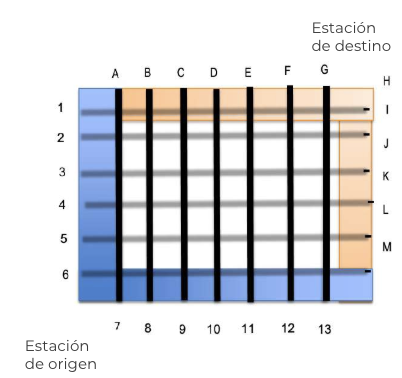
\includegraphics[width=0.25\textwidth]{cuadricula}
	\caption{Ejemplo de cuadrícula}
	\label{fig:3.11}
\end{figure}

\subsubsection{Cálculo de Movimientos}
\begin{itemize}
	\item \textbf{Detección de Cruces:} El robot detecta cruces en la cuadrícula utilizando los sensores QTR, que identifican cuando todos los sensores detectan la línea negra, indicando un punto de intersección.

	\item \textbf{Determinación de la Ruta:} La ruta se determina utilizando las coordenadas de origen y destino. El robot calcula el camino más eficiente evitando puntos bloqueados previamente especificados por el usuario.

	\item \textbf{Actualización de la Posición:} El robot actualiza continuamente su posición en la cuadrícula a medida que se mueve de una celda a otra, utilizando los encoders magnéticos para mantener el seguimiento preciso de sus movimientos.
\end{itemize}

\subsubsection{Movimientos del Robot}
PrimeBot realiza varios tipos de movimientos básicos para navegar por la cuadrícula:
\begin{itemize}
	\item \textbf{Avanzar Una Celda:} El robot se mueve hacia adelante hasta llegar al siguiente cruce.
	\item \textbf{Girar a la Izquierda:} El robot rota 90 grados a la izquierda.
	\item \textbf{Girar a la Derecha:} El robot rota 90 grados a la derecha.
	\item \textbf{Giro en U:} El robot realiza un giro de 180 grados para cambiar de dirección completamente.
\end{itemize}
Estos movimientos son controlados por los motores y ajustados en tiempo real mediante el algoritmo PID para asegurar precisión y estabilidad.

\subsubsection{Representación Gráfica}
PrimeBot genera una representación gráfica de su trayectoria en la cuadrícula, que es visualizada a través de la interfaz serial. La cuadrícula se representa de la siguiente manera:
\begin{itemize}
	\item \textbf{Punto de Salida (S):} Indicado con una 'S' en la cuadrícula.
	\item \textbf{Punto de Destino (D):} Indicado con una 'D' en la cuadrícula.
	\item \textbf{Puntos Bloqueados (X):} Indicado con una 'X' en la cuadrícula.
	\item \textbf{Trayectoria del Robot (*):} Indicado con un '*' en la cuadrícula.
\end{itemize}
La representación gráfica se actualiza en tiempo real para mostrar la posición actual del robot y los puntos recorridos.

\begin{figure}[h]
	\centering
	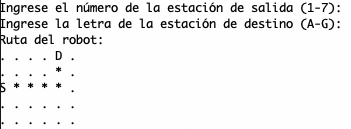
\includegraphics[width=0.50\textwidth]{grafica}
	\caption{Representacion gráfica de la ruta que va a realizar PrimeBot en la Cuadrícula}
	\label{fig:3.12}
\end{figure}

\subsubsection{Parámetros Ajustables por Bluetooth}
Para facilitar el control y ajuste del robot, varios parámetros pueden ser modificados en tiempo real mediante una conexión Bluetooth:
\begin{itemize}
	\item \textbf{Constantes PID (Kp, Ki, Kd):} Permiten ajustar la respuesta del algoritmo PID para mejorar el seguimiento de líneas y la estabilidad del robot.
	\item \textbf{Velocidad Base (BaseSpeed):} Ajusta la velocidad base de los motores para controlar la velocidad general del robot.
	\item \textbf{Coordenadas de Origen y Destino:} Permiten establecer nuevas coordenadas para el punto de salida y el destino, adaptando el recorrido del robot según las necesidades de la prueba.
	\item \textbf{Puntos Bloqueados:} Se pueden definir o actualizar los puntos bloqueados en la cuadrícula, lo que permite al robot recalcular su ruta para evitar estos obstáculos.
	\item El control Bluetooth permite una configuración flexible y rápida, facilitando la adaptación del robot a diferentes escenarios y pruebas del ASTI Robotics Challenge.
\end{itemize}

\subsection{Laberinto}\label{laberinto}

PrimeBot ha sido implementado con la posibilidad de realizar el seguimiento de paredes para poder así resolver laberintos con facilidad.

En resumen, PrimeBot utiliza una combinación de sensores, algoritmos y controladores para calcular y ejecutar movimientos precisos en una cuadrícula, representando su trayectoria gráficamente y permitiendo ajustes en tiempo real a través de Bluetooth para asegurar un rendimiento óptimo en sus tareas de navegación y resolución de laberintos.

